\section{Mosaic Design}

Mosaic is an optimistic bridging solution based on advanced liquidity management, singe sided liquidity pools and a relayer network. At its core it consists of a network of bridges, operated by relayers interacting with smart contracts on source and destination chains. Our proof-of-concept relayer solution is based on a trusted setup, that monitors all connected chains for events, and enacts the transfers accordingly. The next release improves on this model by decentralizing the relayer, using different cutting-edge technologies such as Threshold-Secret-Sharing (TSS) and transaction batching using merkle-proofs. 

The liquidity layer serves to ensure liquidity is moving to the locations where it is needed, allowing the propagation of whatever instructions are required to satisfy the user’s desired outcome, as specified above. We are currently testing this capacity within the EVM ecosystem by running our Proof of Concept (PoC) of Mosaic. From there, we can generalize this liquidity problem and solution to other ecosystems. Liquidity concerns are not new in DeFi. However, they have largely been resolved by automated market makers (AMMs) built into the popular DeFi exchanges like UniSwap and Sushiswap. The introduction of cross-layer and cross-chain applications is, however, making liquidity a more pressing issue than ever before; with so many different layer 2 applications and blockchains to balance liquidity across, and so little infrastructure to do so, liquidity is too siloed for interoperable applications to generate meaningful value.

\subsection{Phase I}

Phase I presents a simple and functional cross-layer solution to enable a transfer system between all major DeFi ecosystems. It is a a Proof-of-Concept with enforced limited functionality to demonstrate the capability of the system.

The main actors in this phase are: an L1 vault in charge of redistributing liquidity, dedicated vaults on each L2, users engaging and providing the required liquidity and a relayer in charge of communicating the different supported networks. All the actors and their interactions are depicted on Figure \ref{fig:v1_mosaic}.

\begin{figure}[h]
    \centering
    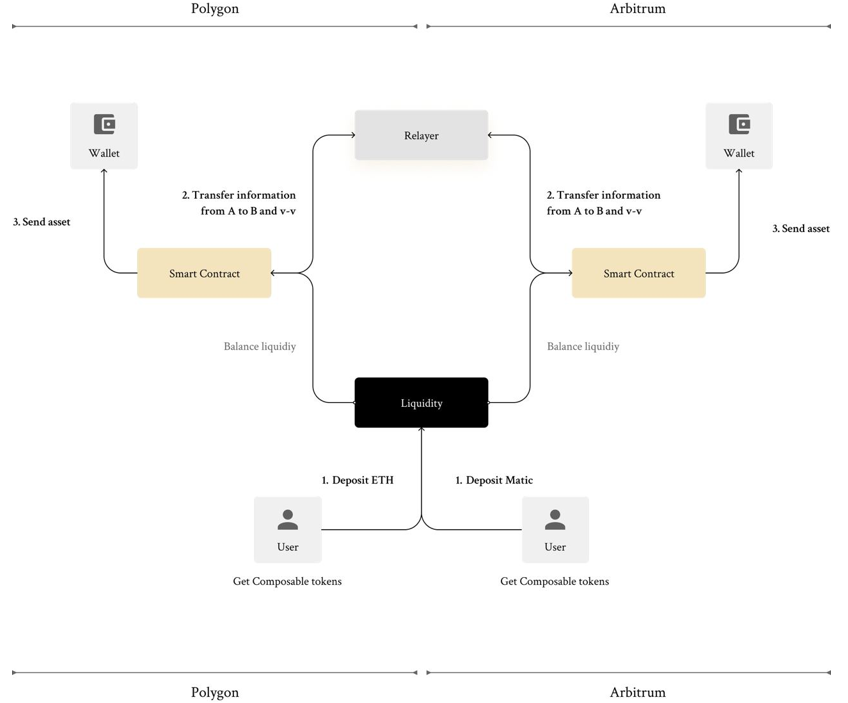
\includegraphics[width=0.75\textwidth]{images/mosaic/v1.png}
    \caption{Polygon-Arbitrum transfer scheme in Mosaic v1.}
    \label{fig:v1_mosaic}
\end{figure}

As you can see on Figure \ref{fig:v1_mosaic}, a transfer consists of 2 important events: the lock event that happens on the source layer and the release event that is triggered by our relayer system on the destination one. This interaction is done on the L2Vault contract, with the lock happening using the \textit{depositERC20} method, while for the asset release, the \textit{withdrawTo} method is called on the L2Vault contract deployed on the other side.

In terms of the necessary liquidity for these actions to happen, users deposit liquidity using the VaultL1 smart contract deployed on L1 mainnet. Users obtain rewards in form of LAYR tokens in exchange for providing liquidity. L1 Vault acts as master with regards the L2 vaults, and redistributes the liquidity on demand. 

By leveraging a lock/unlock pattern on phase I, we were able to proof that interoperability can be obtained in the DeFi space, and that a single curated interface is enough for the user to operate on different layers and chains. We also obtained data about the  user experience and liquidity demands on different networks. Nevertheless, we kept the functionality limited for testing purposes. Thus, we dedicate next phase to enhance and open the protocol to more complex features.
\subsection{Phase II\label{sec:phaseII}}

Phase II represents the evolution of Mosaic v1, our proof of concept. Phase II introduces two main components: a new active/passive liquidity model and a new and more complete set of features that deeply extend the functionality of Mosaic. Phase 2 allows to use different tokens on the source and destination layers, and also introduces the support for new chains such as Moonriver, Fantom, and Avalanche.

\subsubsection*{Active and passive liquidity}
In Mosaic v2 the user has the ability to provide liquidity on any layer and in exchange, besides the APY, he receives receipt tokens that can be integrated with other protocols (e.g: use them as collateral for loans). The user is also able to withdraw liquidity at any point he desires, our dynamic withdrawal fee will calculate the proportional rewards and the user will be credited with the right amount of tokens. Liquidity ca be also directly provided using ETH, and ETH can be transferred among the different layers. In addition to all these new possibilities, we introduce two types of liquidity for different profiles:

    \begin{itemize}
        \item \textbf{Passive liquidity:} In this type of liquidity providing, a more conservative user can obtain some rewards by providing liquidity in his desired layer. It can be understood as staking assets to yield some farm.  On the withdrawal, the user obtains the rewards and recovers the initial liquidity. Passive liquidity can only be withdrawn in the same token it was deposited. 
        
        \item \textbf{Active liquidity:} This liquidity providing model is intended for more knowledgeable and active users with an elevated risk appetite. By leveraging Composable SDK, they can run a dedicated bot to monitor the mempool and  the liquidity requirements of the transactions. If the liquidity of the destination layer is not enough, users can frontrun those transactions in order to gain greater rewards. Active liquidity is specified in number of blocks, and automatically becomes passive liquidity after that time. Active liquidity requires a flowing management but allows users to benefit from unbalanced networks to gain additional yield. Active liquidity can also be withdrawn in any token from any network.
    \end{itemize}
    
\subsubsection*{Cross Layer Function Calls}
Mosaic v2 not only supports value transfers, but also offers cross functions calls. The relayer can transfer the function call and its associated parameters from source to destination in a similar manner as value transfers. To handle calls and returns, it employs a \textit{MsgSender} contract on the source layer, which is in charge of abstracting the user and communicating with the relayer, and a \textit{MsgReceiverFactory} contract on the destination layer. \textit{MsgReceiverFactory} creates \textit{MsgReceiver} instances, which create a virtual identification of the user on the destination network, and interact with the desired protocol. All the interactions on the destination layer are done through the factory contract.

This general architecture, as shown on Fig.~(\ref{fig:crosscall}), allows users to call any protocol on any network and from any source. This elevates Mosaic v2 to a new level of unification, not only value is transferred, but also functionality is bridged together. 

\begin{figure}[H]
    \centering
    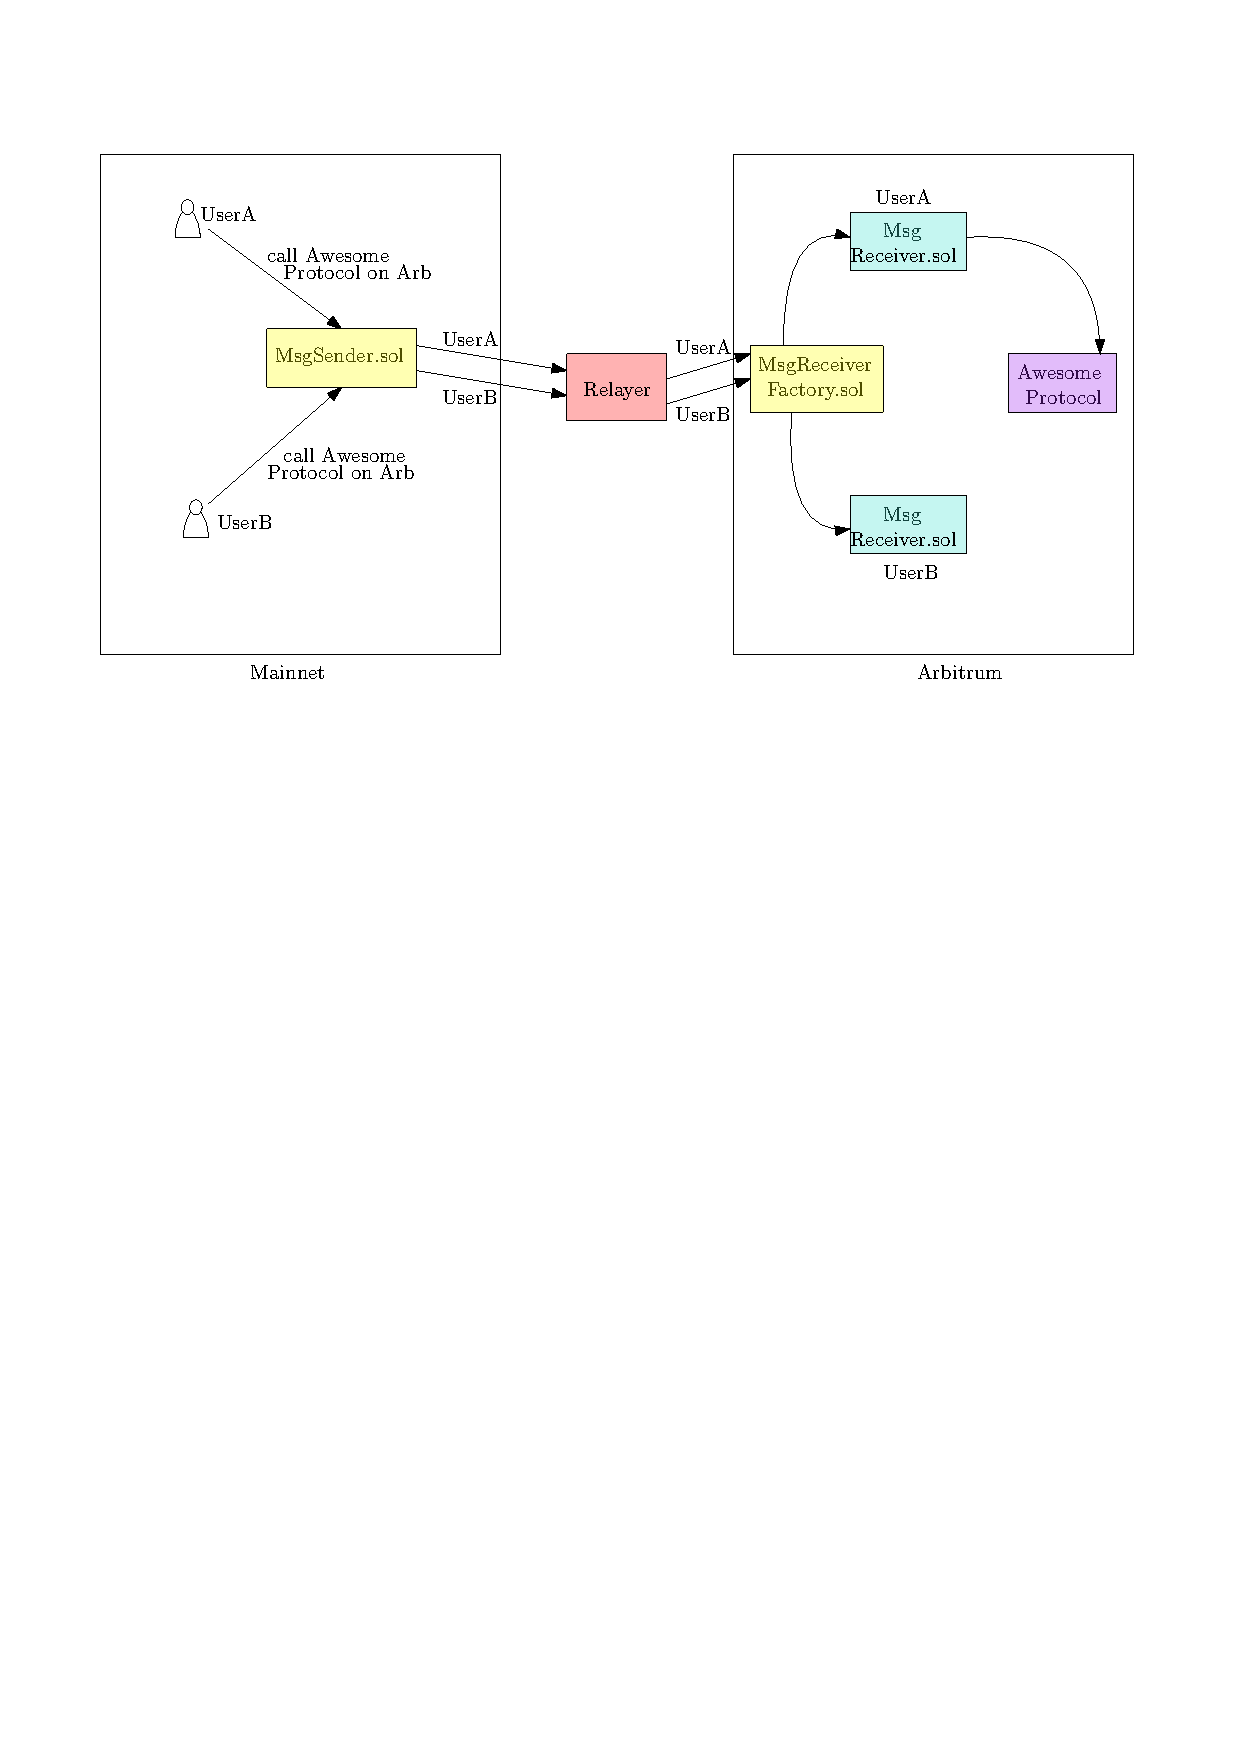
\includegraphics[width=0.9\textwidth]{images/mosaic/crosscalls.pdf}
    \caption{Cross layer function call architecture}
    \label{fig:crosscall}
\end{figure}


\subsubsection*{Other improvements}
In addition to the improvements already mentioned, phase II of the protocol presents the following and varied advances:

\begin{itemize}
    \item Transfer NFTs (ERC-721) between networks by using Ethereum research wrapper proposal \cite{WhyPropertiesb}.
    \item More secure and controlled vaults. Instead of a single \textit{MosaicVault}, everything is isolated in different and dedicated \textit{MosaicHoldings} smart contracts.
    \item Real time liquidity balancing. See Sec.~(\ref{section:lrs}) for more details.
    \item More efficient management of unused funds. Single or combined assets are used to yield farm, resulting in better and more competitive APY for Mosaic's liquidity providers.
\end{itemize}

\subsection{Phase III\label{sec:phaseIII}}

Phase I was about proving a concept and demonstrating that a less fragmented DeFi space was possible. Phase II was about enhancing and increasing the features of Mosaic as well as adding new liquidity models. Phase III is focused on increasing the decentralization of our solution. 

Mosaic’s core consists on a network of bridges, operated by relayers interacting with smart contracts on source and destination chain. Phase I and II are based on a trusted relayer solution, that monitors all connected chains for events, and enacts the transfers accordingly. Phase III improves on this model by decentralizing the relayer, using different cutting-edge technologies such as Threshold-Signature-Scheme (TSS). We allow users to directly participate and monitor in Mosaic's core functionality.

\subsubsection*{RelayerSet}
Each one of the bridges that constitutes Mosaic will be maintained by a group of decentralized and distributed relayers. This set of relayers will manage accounts and smart contracts on both the source and the destination chain. RelayerSets may form a multi-signature account, or use TSS to collectively manage a single private key. The relayers monitor the source chains for XCT requests, and based on the parameters and funds transferred, create the appropriate transactions on the destination chain.

\subsubsection*{RelayerSet Creation}
We’ve chosen to use RelayerSets instead of single relayer nodes to reduce the chance of fraudulent relayers, as well as reducing the stake required to participate as a relayer. In order to increase the security of the RelayerSets, and decrease the risk of a sybil attack, we assign relayers at random to different RelayerSets on-chain.

A user who wants to form part of a relayer group of a given size sends a transaction and initiates the registration. The transaction includes, the identification of the user, the stake he is providing and the size of the TSS he would like to form part of. Algorithm \ref{alg:register_TSS} contains the pseudo-code of the joining process.

    	\begin{algorithm}[H]
			\caption{Register TSS group}
			\begin{algorithmic}[1]
				\Require $t_r \gets \{Stake, msg.sender, size\}$
				\Require groups.  
				\Require needs.
				
				\If{$t_r.Stake < Required Stake$}
				    \State \Return Err
				\EndIf
				
				\If{needs[$t_r$.size] $<$ groups[$t_r$.size] \& $\forall g \in groups[t_r.size] : msg.sender \not \in g$} 
				    \State g $\gets sample(Hash(msg.sender || prev-block-hash))$ 
				    \If{g.size $+ 1=$ $t_r$.size}
				        \State PerformTSS();
				    \Else
				        \If{g.size $<$ $t_r$.size}
				        \State g.size++
				        \State g.append(msg.sender)
				        \State WaitForOthers();
				        \Else
				    	\State \Return Err
				    	\EndIf
				    \EndIf
				\Else
				\State \Return Err
				\EndIf
				\State \Return g
			\end{algorithmic}
			\label{alg:register_TSS}
		\end{algorithm}

\subsubsection*{Staking and Slashing}
In any form of distributed system in which free actors can take part, there is an open door to malicious and/or selfish behaviour. Because every randomly-generated imaginary entity likes money \cite{LightningNetwork}, we need to provide our protocol with a mechanism that punishes malicious actors, while at the same time incentives and rewards honest behaviour.

A stake amount is required to form a RelayerSet, and to individual relayers to join an already established set. The total stake by a RelayerSet sets the budget for their disputable transactions. For a RelayerSet to commit fraud, more than threshold relayers need to commit fraud. For security reasons we may require an elevated percentage of the relayers within a set to contribute in creating a transaction. 

Both TSS and multi-signatures can be used to construct fraud proofs showing which specific relayers colluded, which then leads to a slash of funds on the source chain side. Verification of these fraud proofs is very efficient, as we do not need to prove that a fraudulent transaction was included in the destination chain, only that the relayers signed a fraudulent transaction.

Transactions may be disputed by validators for a certain amount of blocks, we refer to this as the dispute window. As the protocol has Alice submit the transactions for the XCT, both the RelayerSet and Alice need to collude to commit fraud, making the total $slashable_{amount} = funds_{transfered} + relayer_{stake}$. This means that the $funds_{transfered}$ on the destination chain need to remain locked for the duration of the dispute window.

Although $slashable_{amount}$ cannot effectively be reduced; we can unlock the user’s funds earlier, by having liquidity providers stake the $funds_{transferred}$ portion of the slashable amount. An ensurer node operates similarly to a validator (it serve both roles), and observes valid XCTs. The XCT specifies that it wishes a faster unlock on the destination side, and the total fee it is willing to pay for the underlying stake. An ensurer node may then choose to provide the stake for the specified fee. As the insurer node can observe the mempool, source chain, and destination chain state, it is able to determine finality and take the risk that the smart contract cannot. Thus, we provide a faster unlock method to the final user and an opportunity to experienced validators with greater risk appetite to gain additional fees.  An insurer node might be prohibitively expensive for individual users to run. We will provide some way to allow users to provide their assets to a pool, without significant risk.

\subsubsection{Protocol}
We devote this section to give a general overview of how the protocol of Mosaic v3 will operate and how the new RelayerSets integrate on the ecosystem. We also introduce the most common procedures to raise and audit a disagreement during the dispute window.

Let Alice be a user who wishes to transfer an asset from chain Source to chain Destination through a chosen RelayerSet. This cross chain transfer (XCT) consists of a two smart contract interactions; the first on the source chain, which locks assets (XCT-lock), and the second which unlocks funds on the destination layer (XCT-unlock).

Alice initiates the transaction on the source chain, locking the funds in a time locked contract and storing the parameters of the proposed transaction,  then confirms it will relay the transaction by interacting with the contract, which permanently locks the funds. (The confirmation can be negotiated and signed off-chain to reduce gas fees for the relayer).

After XCT-lock has been confirmed, the RelayerSet sends Alice the XCT-unlock transaction, which she commits on the destination chain. Fig.~(\ref{fig:v3_protocol}) illustrates the complete process.

\begin{figure}[h]
    \centering
    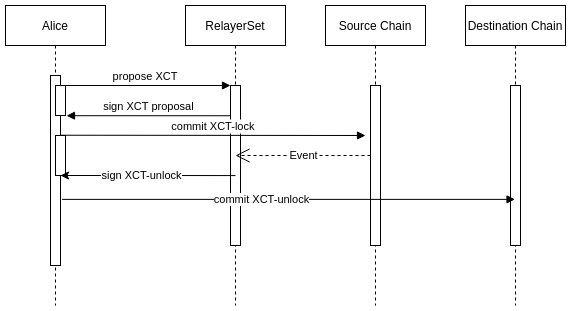
\includegraphics[width=0.75\textwidth]{images/mosaic/phase3/protocol.png}
    \caption{Time interaction scheme of the different actors for a XCT using RelayerSets. }
    \label{fig:v3_protocol}
\end{figure}

\subsubsection*{Disputes}
A malicious RelayerSet can commit fraud in a number of ways, which are handled through on-chain dispute and settled by slashing the stake of the relayers.

    \begin{itemize}
        \item \textbf{Case 1. RelayerSet and user submit a XCT-unlock with no corresponding XCT-lock on the source chain.}
        As illustrated in Fig.~(\ref{fig:dispute1}), when a validator observes a fraud on the destination chain, he musts dispute the RelayerSet on the source and destination chain. Disputes on the source chain are more easily settled since the validator only needs to submit the XCT-unlock event to show the intention of the relayer to commit fraud, independently of the inclusion or finality on the destination chain. 
        
        However, disputes on the destination chain are way more complex since different chains present different finality and consensus models. In order to address this problem, we resort to different proof-of-non-membership that can immediately settle the dispute. If that is not feasible, the dispute may be resolved through decentralized governance.
        
        \begin{figure}[h]
            \centering
            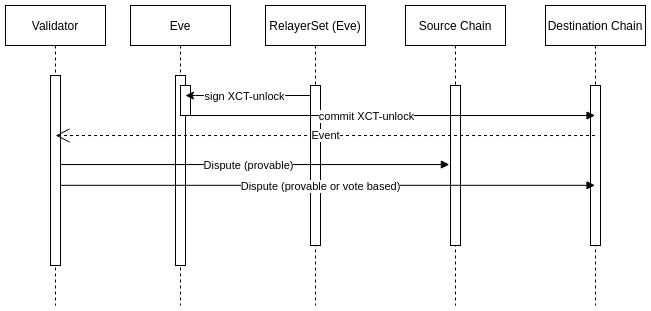
\includegraphics[width=0.75\textwidth]{images/mosaic/phase3/dispute1.png}
            \caption{Time interaction scheme of the dispute resolution when no XCT-lock event is triggered on source chain.}
            \label{fig:dispute1}
        \end{figure}
        
        
        \item \textbf{Case 2. RelayerSet and/or user create a transaction in the destination chain with a different corresponding transaction on source chain.}
        The solution to this dispute is actually identical to the previous one, as there will be no corresponding entry for the transaction on the source chain. Nonetheless, this case will be less common, as the amount of funds lost by the user is greater (the stake + the cost of the XCT-lock transaction), while it does not present additional gains with regards to case 1.
        
        \item \textbf{Case 3. RelayerSet does not create a corresponding transaction on destination chain.}
        Since the RelayerSet confirms on the source chain that it will relay by signing the XCT proposal, the fraud proof becomes showing the destination chain that RelayerSet committed to signing an XCT-unlock. The user can then re-obtain their funds on the destination chain. The proof is depicted in Fig.~(\ref{fig:dispute3}).
        
        \begin{figure}[h]
            \centering
            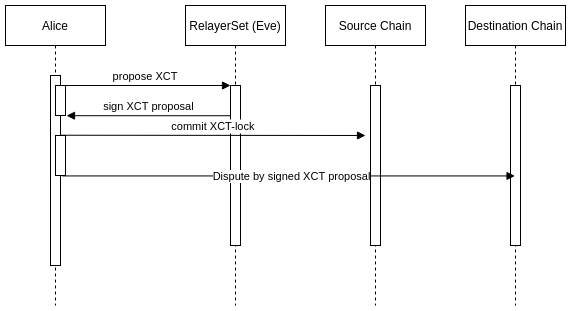
\includegraphics[width=0.75\textwidth]{images/mosaic/phase3/dispute3.png}
            \caption{Time interaction scheme of the dispute resolution when no transaction is created on destination chain. }
            \label{fig:dispute3}
        \end{figure}
        
        In the case where an honest RelayerSet provides XCT-unlock, but the user does not submit the transaction, the RelayerSet may still submit the XCT-unlock transaction during the dispute window and slash funds from the XCT.
        Not all destination chains may support smarts contracts. In that case; it must be possible to construct a proof of (non)-inclusion for the destination chain. The user then re-obtains their funds on the source chain.

    \end{itemize}


\subsubsection{TSS vs Multi-signatures}

In a decentralized and distributed environment, we need a mechanism that allows for verification, integrity and non-repudiability of messages. The most common tool for this goal is the use of digital signatures. Digital signatures are an instrument of public key cryptography \cite{Diffie1976NewCryptography} that allows for public verification. Multiple signatures schemes exist, most of them are based on the initial standard of DSA \cite{DSSStandard} and can be summarized as the following set of algorithms:

\begin{itemize}
    \item Key generation$(1^{\lambda}) \rightarrow (sk,pk)$. As the algorithm that takes as input a security parameter $\lambda$ and produces the signing key $sk$ and the public verification key $pk$.
    
    \item Signature$(m, sk) \rightarrow \sigma$. Which is the algorithm that takes a message $m$ and the signing key $sk$ to produce a signature $\sigma$.
    
    \item Verification$(pk,\sigma, m) \rightarrow 1/0$ As the verification algorithm that takes the message $m$ and the signature $\sigma$ and verifies them using the public key $pk$. It outputs a boolean with the result of the verification.
\end{itemize}

For our cross-chain solution, we consider two well-known and established schemes: multi-signatures and TSS. Both schemes serve our purpose of redistributing the responsibility among a set of parties, but there are some key differences we summarize here. 

\begin{itemize}
    \item \textbf{Multi-signature:} As the name suggest, it is a scheme that involves multiple signatures. To be considered valid, different parties need to sign the same content. It can be architectured in a threshold manner such that a minimum of signatures is required to be considered valid (e.g: 2-out-of-3). It produces as many signatures as the set of parties involved.
    
    \item \textbf{TSS:} Threshold Signature Schemes \cite{Gennaro2019FastSetup, Canetti2021UCAbortsb} are a special kind of signatures that allow to redistribute the responsibility between a set of parties. In a TSS, the secret key is not known by any party, each party has a partial secret key, and needs to collaborate with the a minimum subset of the parties (e.g: 3-out-of-5) in order to produce a valid signature. Only one single signature is produced and there is no difference on the signature produced or the verification process, when compared to traditional signatures.
\end{itemize}

Both approaches have its benefits and drawbacks. On the one hand, multi-signature is easier to implement since it is based on independent signatures and requires no additional setup. However, it produces multiple signatures, increasing the costs on the blockchain and the verification times, since each individual signature needs to be separately verified.

On the other hand, TSS  require quite a complicated setup, with multiple sub-protocols and the use of homomorphic cryptography \cite{Moore2014PracticalSurvey}. Nonetheless, the verification is simpler and faster than the multi-signature scheme. A simple scheme of both signatures protocols is depicted in Fig.~(\ref{fig:signatures}).

\begin{figure}[H]
    \centering
    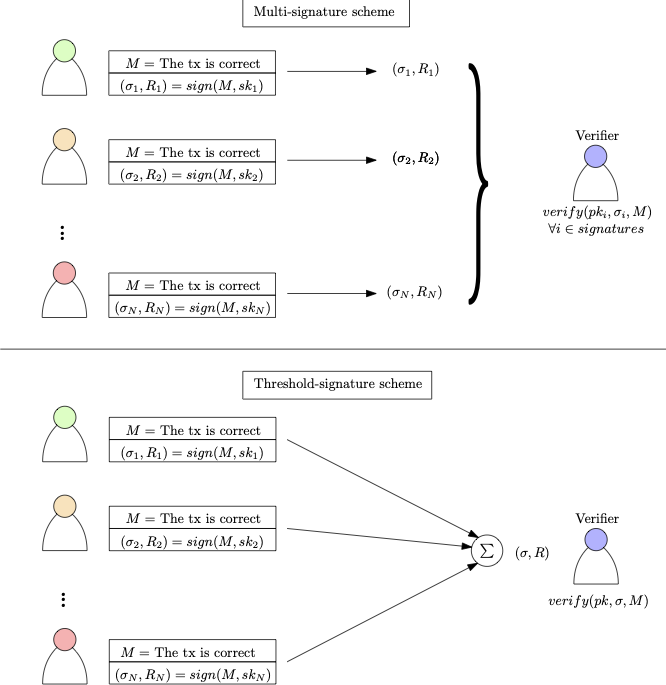
\includegraphics[width=0.9\textwidth]{images/mosaic/phase3/signatures.png}
    \caption{Multi-signature vs. TSS. Here, $\sigma$ represents a partial or complete signature, $R$ is the randomness used in the process, $M$ represents the message to be signed and $sk_i$ illustrates their partial or personal secret key.}
    \label{fig:signatures}
\end{figure}


Since we are focused an interested on keeping the operational costs as lower as possible for the user, we choose the TSS scheme. The setup can be performed off-chain, and then only a single signature and public verification key need to be broadcasted. This keeps the blockchain transaction and storage costs to a minimum while leveraging and state of the art signature scheme with all the desired security properties.


\subsubsection{Alternative model}
We presented the the protocol, the dispute resolution engine and the cryptographic constructs that enable Mosaic v3. However, there exist an alternative model we have also considered. In function of the data we gather from Phase II, we might consider this secondary approach. For the sake of completeness, we briefly describe the second model we considered.

As other projects have explored \cite{HopRollups, MOVRMOVR}, when a common layer or chain is available (e.g: L1 on Ethereum and RelayChain on Polkadot), cross-chain transfers can be achieved by bundling different transactions. The state (e.g: transactions or messages) from a source chain is transferred to the destination chain in a cryptographic accumulator, usually in the form of a Merkle Root \cite{Becker2008MerkleCryptanalysis}. As depicted in Fig.~( \ref{fig:accumulator}), the state is comprised on source chain and sent to the destination chain through the common layer. Later on, by proving membership  and unpacking the Merkle root, messages can be recovered on the destination layer.  By bundling information, we can reduce transaction costs on the common layer as well as benefiting from its security since the whole process is done on-chain. To ensure the validity of data being transferred, some stake is locked or an optimistic approach is pursued until the source chain settles its sates on the common chain. Then, the data is considered final and can be used as ground truth.

\begin{figure}[H]
    \centering
    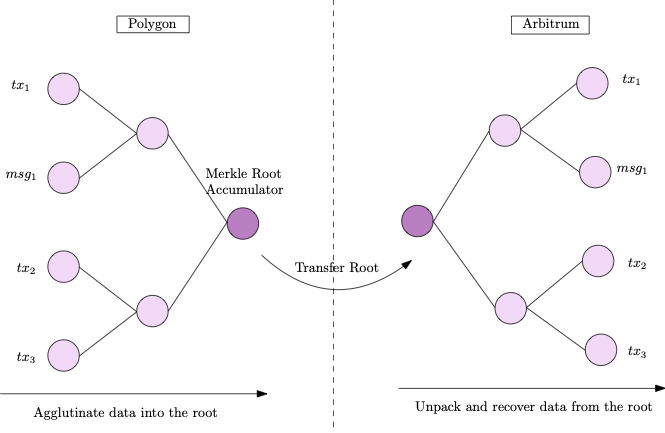
\includegraphics[width=0.9\textwidth]{images/mosaic/phase3/accumulator.png}
    \caption{Accumulate and transfer scheme. Only the Merkle root is transferred on-chain to  reduce costs.}
    \label{fig:accumulator}
\end{figure}

We believe Mosaic is more general than this approach, since it does not depend on the existence of a common layer and replaces the finality gadget with a set of decentralized relayers. Nonetheless, we might consider this agglutination scheme for scenarios in which a common layer can be easily found, in an effort to keep as much of the process on-chain. Please note that this approach still requires, to a certain degree, off-chain services in order to operate properly.
\subsection{Liquidity Simulation Environment\label{section:lse}}

As part of building Mosaic \cite{MosaicFinance} we wanted to understand the nature of liquidity and how its allocation and movement means for the design of the system.
%
To that end, Composable Labs \cite{IntroducingMedium} built a Liquidity Simulation Environment (LSE) \cite{IntroducingMediumb}.

This software tool can simulate allocations of assets to vaults and assets moving around in the network.
%
It is modular and you can produce data in any form you want.
%
Currently, the LSE supports data generated from a truncated Gaussian, Geometric Brownian Motion (GBM), and data sampled from our 2021 September-October PoC run \cite{TestingMedium}.

The strategy layer allows for any liquidity allocation and movement approach to be defined. For example "move liquidity from vault X to vault Y when conditions Z is true".
%
An objective - which can also be defined in the LSE - useful for searching for the best strategy could be to optimize the liquidity distribution among the vaults so that any transfer can be supported.

Fee models, how much and simply how, to charge moving assets can be defined as well. In fact, we used the PoC in conjuncion with the LSE to decide the best fee model to use in the context of available data up to that point.

The LSE is built as a state-machine iterating through the simulated transfers changing the states of the vaults. Replenishment events can be triggered - for example: the Arbitrum vault needs liquidity from the Mainnet vault.

The LSE is also continuously improving. As more transfer data is received this gives us a unique insight into how Mosaic is used and the LSE can help fine-tune our network to achieve an optimal user experience by having maximum availability.

\subsubsection{Simulating Data}

The LSE supports generating simulated transfer/usage data. We use this to model behavior of network usage and based on that make decisions on how to distribute liquidity.

We support generating data from a truncated Gaussian distribution. We sample a timeline and on that a set of hypothetical cross-chain cross-layer moves from this distribution with given mean and standard deviation.
%
We also support generating data from a Geometric Brownian Motion.
%
The moves or transactions $N_t$ (amount of \$) from one vault to another, at time $t$, following a GBM model, are described by the following stochastic differential equation (SDE)
\begin{equation}
\frac{d N_t}{dt} = \mu N_t + \sigma N_t\frac{dW_t}{dt}, 
\end{equation}
with $\mu$ being a drift term, $\sigma$ the volatility, both assumed to be constants and $W_t$ is a Brownian motion stochastic process. The analytical solution of the above SDE at time t, given initial condition $N_0$, is known to be 
\begin{equation}
\label{eq:gbm_solution}
N_t = N_0 \exp\left[ \left(\mu - \frac{\sigma^2}{2}\right) t + \sigma W_t\right],
\end{equation}
which by definition is always strictly positive. A key property of the solution, important for our LSE use, is that the solution asymptotically goes to infinity when $\mu > \frac{1}{2}\sigma^2$, it goes to $0$ when $\mu < \frac{1}{2}$ and it fluctuates between zero and arbitrarily large values when $\mu = \frac{1}{2}\sigma^2$, therefore for most of our cases we will be using $\mu = \frac{1}{2}\sigma^2$. Fig. \ref{fig:gbm} shows two random simulation of eq. (\ref{eq:gbm_solution}) for the $N_0 = \$2000$, $\sigma=2$ and $N_0=\$1500$, $\sigma=1$ respectively. Note that the same initial and volatility values have also been used in our simulations below to simulate moves from Polygon to Arbitrum vaults and vice versa.
%
\begin{figure}[h]
    \centering
    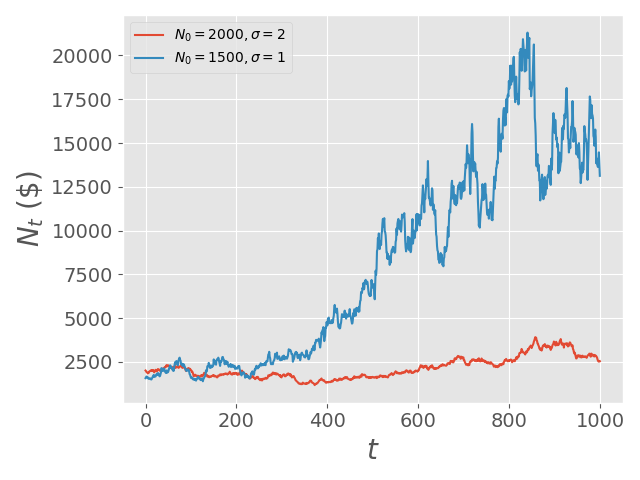
\includegraphics[width=0.5\textwidth]{images/gbms.png}
    \caption{Simulation of Geometric Brownian motion data in Composable's Liquidity Simulation Environment (LSE).}
    \label{fig:gbm}
\end{figure}
%

These results guided us to an answer on two key questions to kick off the Mosaic PoC: First, how much liquidity should be assigned in total and then how much should be assigned to each network? Second, which transfer fee model should we initially use?

These results guided us to decide on a good initial fee model to use for the Mosaic PoC. We then ran the PoC with that model, collected the data, and optimized the model to its final form. More on that in Sec.~(\ref{sec:feemodel}).

\subsubsection{Mosaic Fee Model\label{sec:feemodel}}

One of the first use-cases of the LSE was deciding which fee model to use for Mosaic.
%
Fees are charged when funds are moved between networks. The question of which fee model to go with is key to a successful deployment.

First, guided by Occam's razor \cite{WhatRazor} we picked a simple functional form and let the fee model follow a linear form capped by a maximum fee ensuring that nobody, no matter how much they move across Mosaic, is charged more than a certain percent.

For most transfers, and for practically all retail transfers, users move along the linear part close to the origin.
%
To ensure a safe network, we implemented a minimum fee as well distributing rewards to maintainers. Let $x$ denote the liquidity moved as percent of available liquidity in the origin vault. For example, if I move 10 ETH in a vault with 200 ETH $x=5$\%. Let $y$ be the fee charged in percent. The Mosaic fee model is then determined by the two points $(x,y)=(0,0.25)$ and $(x,y)=(30,5)$.

The Mosaic PoC was run with this model and based on the data the two points were optimized to balance use and network safety (indirectly via rewards collected from fees).

We have three free parameters in our fee model:
\begin{itemize}
    \item the liquidity-\% at which the maximum fee kicks in (also called $a$)
    \item the maximum fee \% to charge
    \item the minimum fee \% to charge
\end{itemize}

In the PoC these parameters were: 40\%, 4\%, and 0.25\%, respectively. For ease, we will denote this parameter set in the format (40, 4, 0.25).

The PoC transfer data is visualized in Fig.~(\ref{fig:pocdatavis}).
%
\begin{figure}
    \centering
    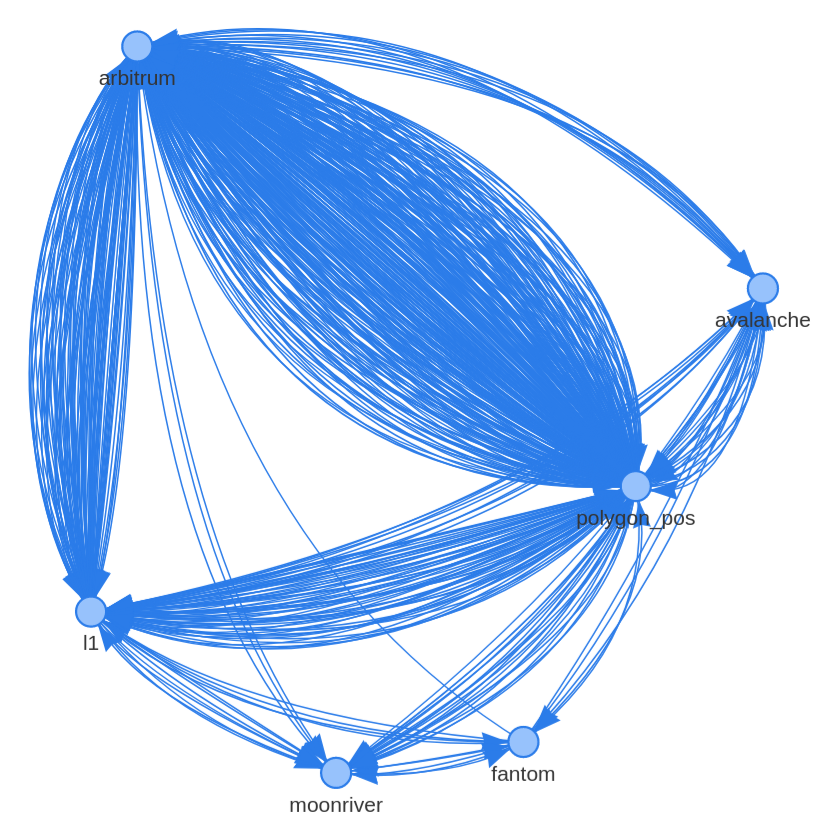
\includegraphics[width=0.6\textwidth]{images/mosaic/pocdata.png}
    \caption{Visualizing the Mosaic PoC bridge transfer data. Each network supported by Mosaic in the PoC is a node and edges represent transfers between the networks. Note that Arbitrum and Polygon were there from the beginning and other networks were added later. Thus, edges are not normalized by time and surely does not imply "popularity" of a network.}
    \label{fig:pocdatavis}
\end{figure}
%
We next visualize the fees charged for the PoC data in Fig.~(\ref{fig:pocdatafees}).
%
\begin{figure}
    \centering
    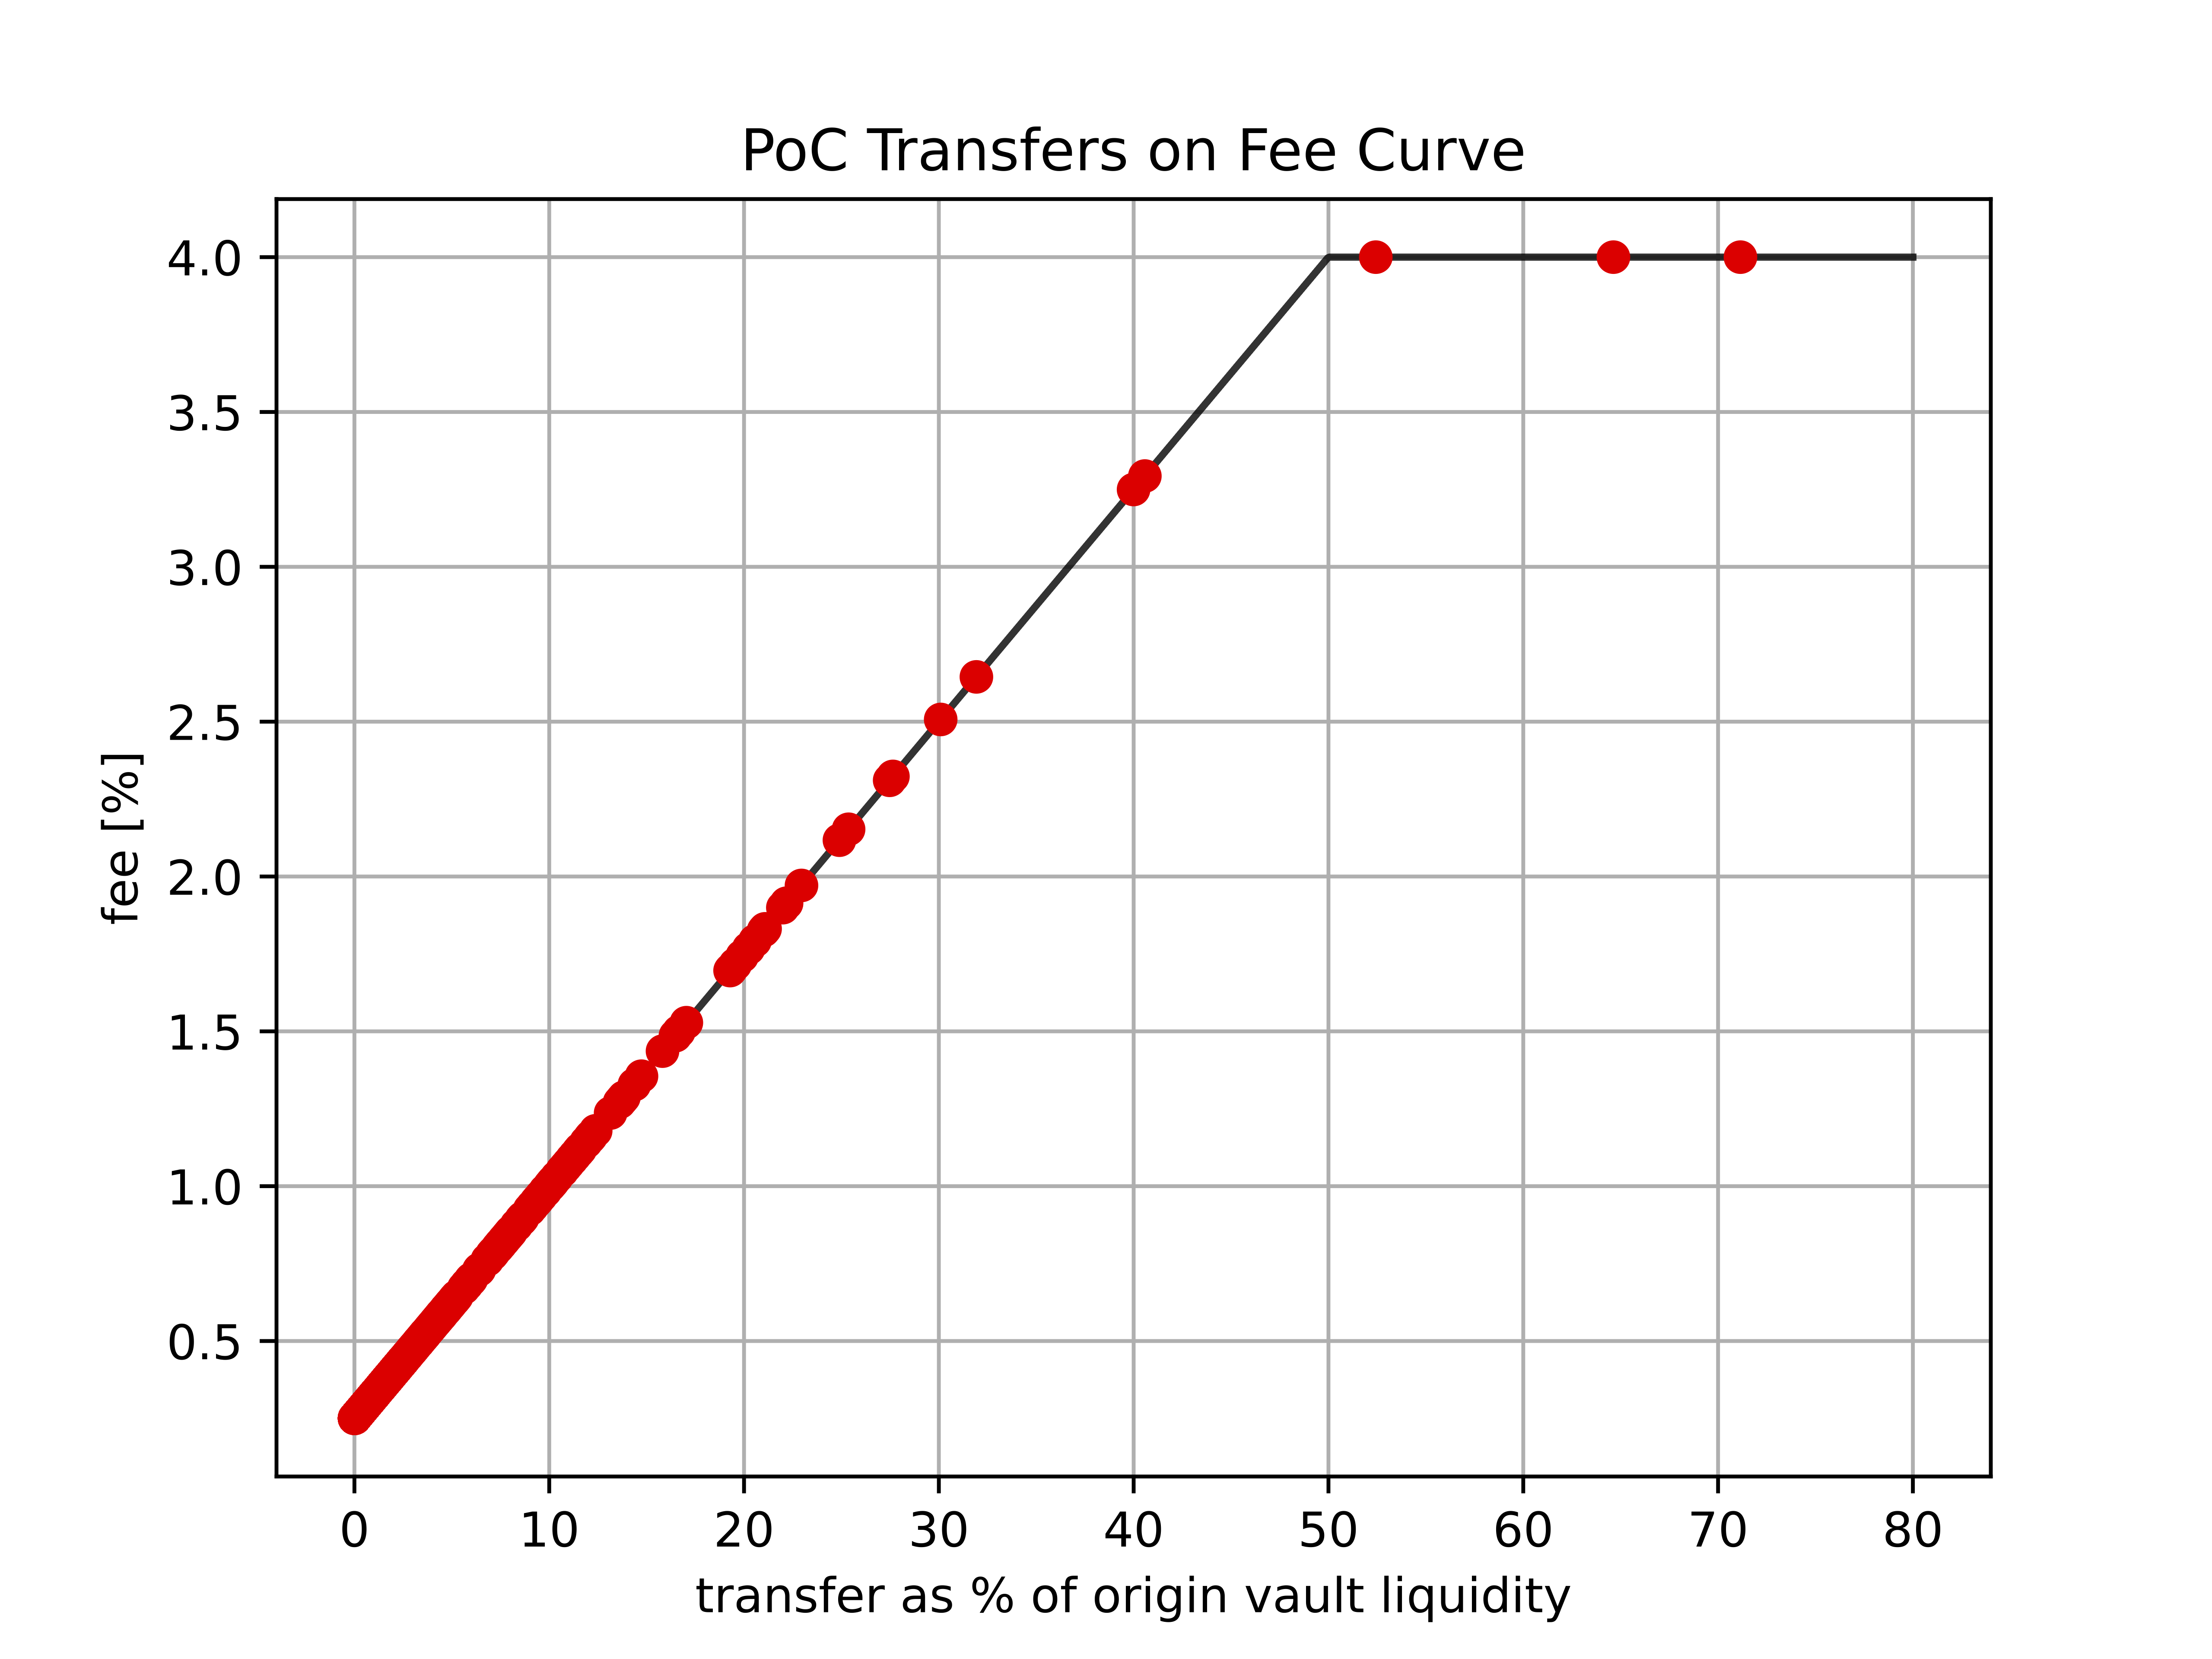
\includegraphics[width=0.8\textwidth]{images/mosaic/poc_transfer_on_fee_curve.png}
    \caption{Fee charged vs transfer amounts as percent of available liquidity in the origin vault. For example, if 10 wETH is transferred from a vault on Arbitrum with 1000 wETH it would show up at $x=10$\%. The y-axis shows the fee charged for the transfer. For the PoC vaults were on the order of \$100-200k at the beginning of the PoC. The exact numbers for each token (which in turn was distributed across multiple networks like Arbitrum and Polygon) are available here: \href{https://mosaic.composable.finance/earn}{TVLs for Mosaic} (accessed November 12, 2021).}
    \label{fig:pocdatafees}
\end{figure}
%
To decide on a good set of parameters, we next compare this to bridges seen in the general cross-ledger community.

We find that some operators charge a fixed 0.5\% for all transfers, higher than the average Mosaic PoC case.

Other operators charge different fees depending on whether you are leaving Ethereum or arriving from another chain. Some charge a fixed dollar amount and others a percentage with minimum and maximum dollar amounts.

Some operators do not charge a fee but instead charge a ``hidden fee" by quoting a given ``transfer rate". They also create bi-directional fees (mainnet to polygon is different than polygon to mainnet).
%
Other operators charge a fee that is a multiple of the destination network fee.

And so on.

Given this landscape of fees the following parameters were chosen: (30, 4, 0.25) (liquidity-\% at which max fee kicks in, maximum fee \% to charge, minimum fee \% to charge, respectively).
%
This optimized fee curve is shown in Fig.~(\ref{fig:pocdatafeesopt}).
%
\begin{figure}
    \centering
    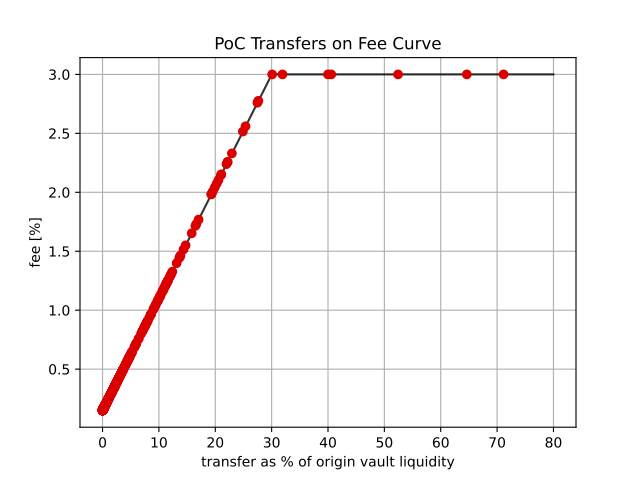
\includegraphics[width=0.8\textwidth]{images/mosaic/poc_optimized.png}
    \caption{The PoC data transformed to the optimized fee curve with parameters (30, 4, 0.25).}
    \label{fig:pocdatafeesopt}
\end{figure}
%

\subsubsection{Continuous Improvement}

With the LSE we can continuously collect data from the operation of Mosaic and periodically revisit the fee model parameter settings.
%
This introduces us, as shown, to a purely data driven approach to determine this. We would use Graph QL \cite{GraphQLAPI} to collect data from the Mosaic network, compute the fees/revenues collected and ensure that we stay within a certain band of expected and allowable values. We make this check once a week.
%
If we stray away from expected values, we modify the parameters if necessary based on a data review.

\subsection{Liquidity Rebalancing System\label{section:lrs}}

The best user experience is obtained when the liquidity availability is high thus allowing, in general, any token to be moved from any network to any other network.

To that end, we used the LSE from Sec.~\ref{section:lse} to design a forecasting and rebalancing technology which can predict in advance when a certain liquidity level will be reached for a given vault. This is built into Mosaic.
%
It is critical for the optimization of the passive liquidity rebalancing that will enable passive liquidity providers to continue to service cross-layer transfers.
%
Having an optimal allocation of capital across layers is key to offering the best performance for users seeking to move cross-layer. Therefore, understanding when said capital reaches certain key levels where action will need to be taken is important.

More formally, enter the Liquidity Rebalancing System (LRS) developed by Composable Labs.
%
\begin{figure}
    \centering
    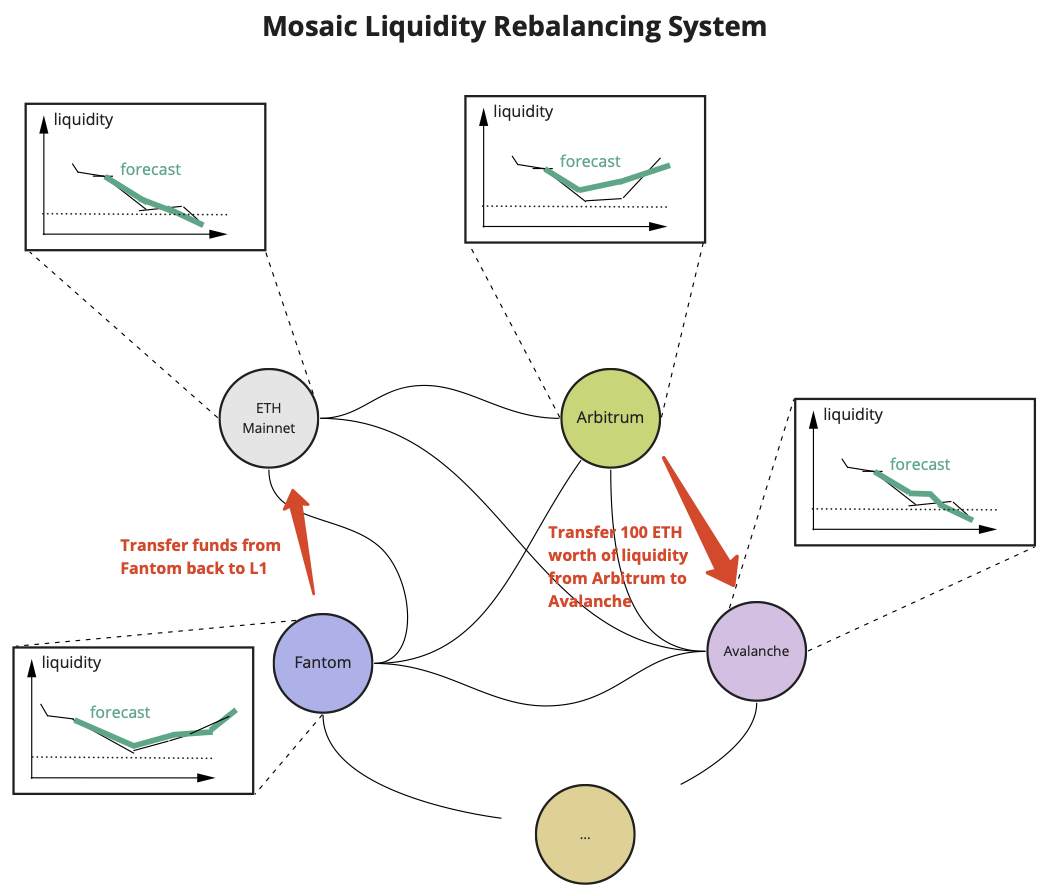
\includegraphics[width=0.9\textwidth]{images/lrs.png}
    \caption{Sketch of the Liquidity Rebalancing System showing how a forecast model is built on the liquidity in each vault in the Mosaic network. Transfer of funds are moved as needed when a subset of vaults are depleted (to a certain pre-set level, we use 90\% here which is conservative) needing funds from a donor vault.}
    \label{fig:lrs}
\end{figure}
%
In Fig.~(\ref{fig:lrs}) we show a graph of various networks such as the Ethereum mainnet, a layer 2 solution Arbitrum, Avalanche, and Fantom, but Mosaic supports many more networks and is growing.

LRS builds a forecasting model on each network (shown as the insets with black lines being the liquidity data and green lines being the forecast model). At a given frequency, e.g. hourly, it checks the status of all networks, computes where liquidity is needed and performs the transfers.
%
The transfers take place as follows: if a vault is predicted to be depleted to 80\% of its seed amount then funds are moved from a so-called ``donation" vault. If a vault has too much liquidity, or satisfy a broader set of metrics to be defined later, it becomes a donation vault (this status is temporary).

The system overall consists of two key pieces: First, we have a forecasting model predicting the evolution of liquidity in a single vault on a single network and second, we have a broader logic deciding how to distribute available liquidity across the entire connection of networks (a connected graph).

\subsubsection{Forecasting a Single Network}

To forecast a single network we developed multiple models starting with a set of baseline models including an autoregressive integrated moving average (ARIMA) model \cite{AnScience}, Holt's linear trend model (HLT) \cite{7.2Ed}, and a Holt-Winters seasonal method \cite{7.3Ed}. We will show the ARIMA and HLT performance in what follows.

Also, the eventual goal is to build Artificial Intelligence (AI) \cite{ArtificialBritannica} based models such as long short-term memory (LSTM) \cite{UnderstandingBlog}.
%
This work is in the pipeline and the non-AI baseline models will help us compare and also develop a two-tiered system where non-AI and AI work to forecast together.

\subsubsection*{Forecasting with ARIMA}

To simplify the discussion and without loss of generality we assume a graph of three networks: L1, Arbitrum (ARB), and Polygon (POL).
%
We first develop an ARIMA model to fit and forecast liquidity data on the POL vault, that can be mathematically described as 
%
\begin{equation}
    Y_t - \alpha_1Y_{t-1} - \dots - \alpha_{p'}Y_{t-p'} = \epsilon_t + \theta_1\epsilon_{t-1} + \dots + \theta_q\epsilon_{t-q},
\end{equation}
%
where $Y_t$ is our time series data at discrete time $t$. Although the above expression applies to the more widely known \emph{autoregressive moving average} (ARMA) \cite{TimeScience} models with $p'$ and $q$ being the orders of the autoregressive (AR) and moving average (MA) terms, here we also account for the fact that non-stationary effects are present in our data and, therefore, a differencing step needs to be applied to the data prior to fitting the model.
%
The order of the differencing step depends on the multiplicity of the unit root. Using the lag operator notation, $L^i[Y_t] := Y_{t-i}$, the times series model can be written as 
%
\begin{equation}
    \left(1 - \sum_{i=1}^{p'} \alpha_i L^i\right) Y_t = \left(1 + \sum_{i=1}^p\theta_i L^i\right)\epsilon_t
\end{equation}
%
and in the presence of a unit root with multiplicity $d$ we have 
%
\begin{equation}
    \left(1 - \sum_{i=1}^{p} \phi_i L^i\right) (1 - L)^d Y_t = \delta + \left(1 + \sum_{i=1}^p\theta_i L^i\right)\epsilon_t
\end{equation}
%
representing the ARIMA(p, d, q) process.

Next, we developed an automated model selection of the ARIMA order parameters such that the rebalancing system does not require manual input to determine its parameters when a dataset is provided.
%
Below we are presenting a list of criteria that we have used in order to identify the optimal order of differencing $d$ in the data and the orders of autoregressive and moving average terms, $p$ and $q$, in the ARIMA(p, d, q) model. 

\subsubsection*{Identifying the order of differencing in the data}

The first step in fitting an ARIMA model is the determination of the order of differencing needed to ``stationarize" the series. Normally, the correct amount of differencing is the lowest order of differencing that yields a time series which fluctuates around a well-defined mean value and whose autocorrelation function (ACF) plot decays fairly rapidly to zero, either from above or below. If the series still exhibits a long-term trend, or otherwise lacks a tendency to return to its mean value, or if its autocorrelations are positive out to a high number of lags (e.g., 10 or more), then it needs a higher order of differencing. Although the presence of most of these characteristics can be observed by simply looking at the differenced data plots, in order to automate our model selection procedure, we work primarily with the autocorrelation function.

The first rule that we apply is that, if the series has positive autocorrelations out to a high number of lags, then we increase the order of differencing by one. 
A sign that can often indicate that the time series might be overdifferenced is to observe an lag-1 autocorrelation that is below $-0.5$. In practice, in order to apply these two rules, we fit an ARIMA(0, d, 0) model, that is a model with no AR or MA terms, but only a constant term which when trained, it provides an estimate of the mean of the data. Thus, the residuals of this model is simply the deviation from the mean. Once we identify a sufficient $d$ such that the aurocorrelation function drops to small values past lag-1, we also compare the resulting model with an ARIMA(0, d+1, 0). Assuming that lag-1 autocorrelation does not fall below $-0.5$ (which would be a sign of overdifferencing), if the model with d+1 order of differencing exhibits lower standard deviation values then it is preferred over $d$, otherwise we keep $d$ and we proceed with the selection of optimal $p$ and $q$ orders. 

\subsubsection*{Identifying the AR(p) and MA(q) orders}

Next, in order to identify the number of autoregressive and moving average terms, we proceed as follows: 
For the number $p$ of AR terms we set it equal to the number of lag terms that it takes for the partial autocorrelation function (PACF) to cross the significance limit.
%
Similarly, the number $q$ of MA terms, we use the autocorrelation function (ACF) instead and it is set again equal to the number of lag terms that it takes to cross the significance limit. 

\subsubsection*{Optimizing the ARIMA model for our LSE data}

In what follows we employ our model selection capability explained above to optimize our ARIMA model parameters and use them for forecasting.

We generate simulated data with the LSE. Our time series data consists of $1000$ liquidity transfer observations obtained on a hourly basis ($\Delta t = 1$ hour).
%
We briefly touched on how these are computed, but let us provide more details here. We select a number of token movements of the vaults. These are drawn from a truncated Gaussian with parameters set to resemble real-world transfers. As an aside, the Mosaic PoC provided even more realistic data and we have developed ways to account for this as well - we are able to confirm that our simulated data resembles the PoC data.
%
Then, the simulated data is snapped to a global timegrid and a state machine is used to evolve the vault states forward starting at some initial liquidity levels. This give rise to the evolving liquidity levels over time as plotted in Fig.~(\ref{fig:lse_datasets}).

\begin{figure}
    \centering
    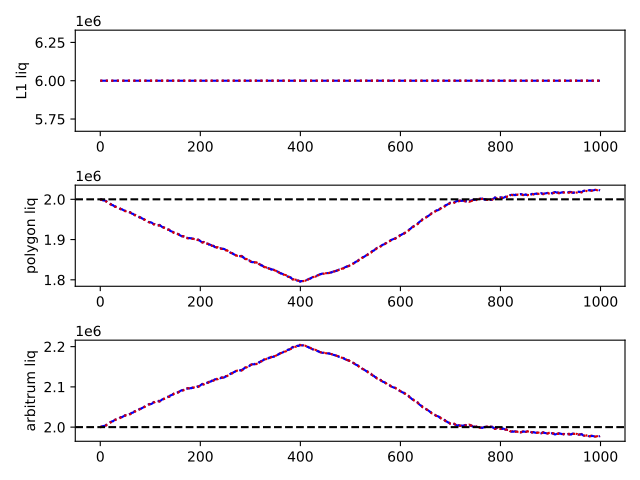
\includegraphics[width=0.49\textwidth]{images/lse_results_feemodel_3_20_20211015_18_59_40_412997.png}
    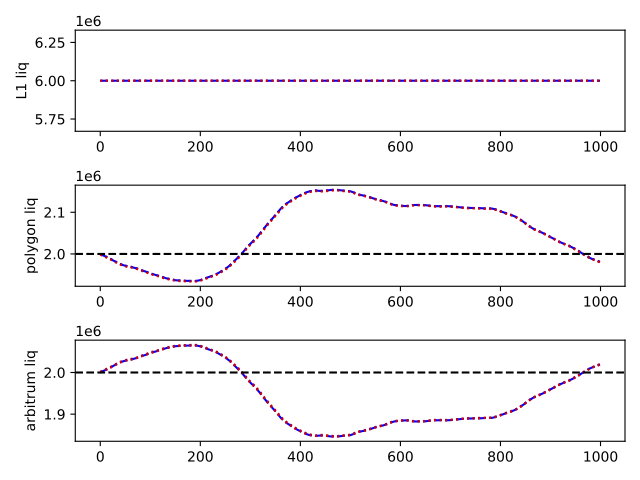
\includegraphics[width=0.49\textwidth]{images/lse_results_feemodel_3_20_20211021_18_59_52_314364.png}
    \caption{Dataset 1 (left) and Dataset 2 (right) from the Liquidity Simulation Environment (LSE). Each vault is a row. The liquidity is shown as the moving curves in rows 2 and 3. Row 1 does not have transfers involved with it for this data.}
    \label{fig:lse_datasets}
\end{figure}

We use $200$ training points (roughly 8 days worth of data) each time we fit an ARIMA model and we use it to forecast on a time horizon of $168$ hours; roughly 1 week ahead which coincides with some layer 2 to layer 1 exit times.

Then, we run the model selection algorithm every time we shift the time frame 10 time steps ahead, and we find that in all cases the number of AR terms varies from $3$ to $6$ while the optimal number of MA terms is always $1$ for both Datasets 1 and 2.

We next show the performance of the ARIMA model as well as of HLT. In the HLT approach, also known as double exponential smoothing, we identify a linear trend in the time series and make a prediction using the smoothed value $s_t$ and the linear trend term $b_t$ at time $t$.

See the forecasting comparison and performance for the Arbitrum vault in Fig.~(\ref{fig:arb_conserv}).

\begin{figure}[h]
    \centering
    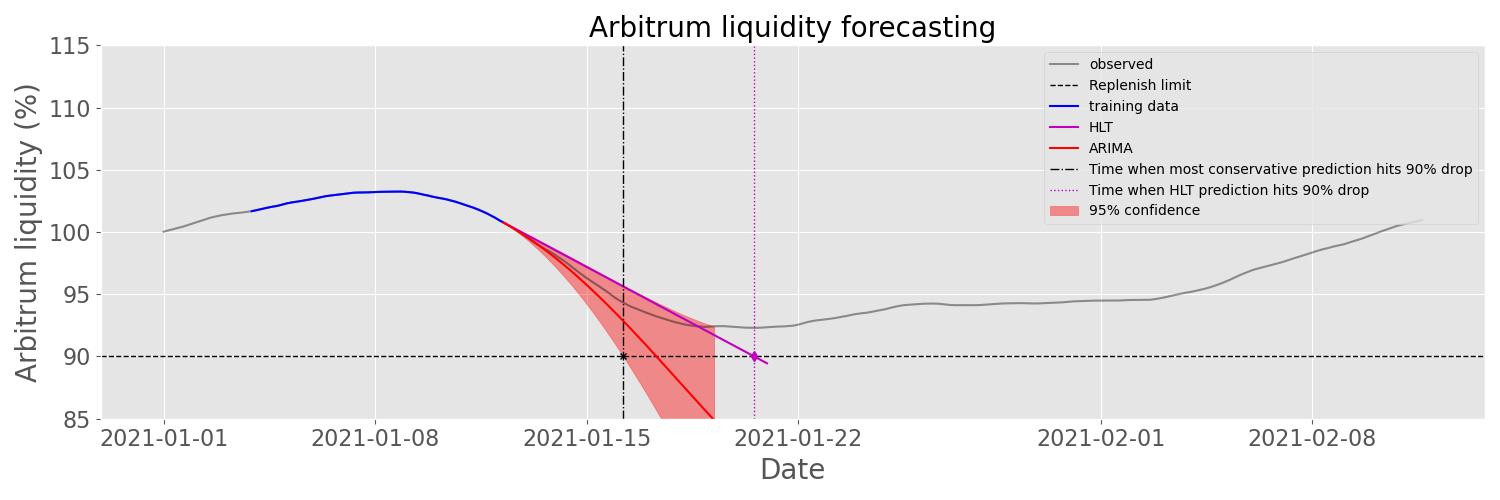
\includegraphics[width=\textwidth]{images/arbitrum_instance_t_fin270_90perce_drop.png}
    \caption{Forecasting comparison between ARIMA and HLT models. The black point shows when the ARIMA model predicts that a 90\% liquidity level is reached in the vault - by conservative estimates (the lower confidence level). The purple point shows when the HLT model predicts the same 90\% liquidity level. While both predictions can be used to trigger, in advance, a replenishment event, the ARIMA predictions appears to be much more conservative.}
    \label{fig:arb_conserv}
\end{figure}

We run a forecasting model on each vault and this, in turn, triggers the rebalancing system to move liquidity accordingly to always keep the vaults ready and liquid thus maximizing the successful transfer rate.

We note that, as we run the forecasting model across the data in a rolling window fashion, the data is contained within the 95\% confidence bands in the amount of time expected allowing us to perform accurate and conservative replenishment event estimates.

\subsubsection{Rebalancing Logic}

With a forecasting model built on each network, the next step is designing the rebalancing logic of the overall system.
%
Here is our approach. At a given cadence which can depend on transfer activity in the general network, we check the following: First, what is the set of current liquidity donation vault. We assign a score to each vault and sort them. For each donor, we also log how much liquidity can be donated.
%
This implies that we have a list of candidate liquidity donors.
%
Next, we obtain the list of vaults which are in need of liquidity. Perhaps this is an empty set, but assuming not, we simply deplete as much liquidity from the donors going top down until all liquidity has been rebalanced.

The score assigned to a vault in the ``donor detection phase" is determined based on a set of metrics including: how active is this vault (inactive implies that it can donate without needing liquidity itself), how much ``active" liquidity is assigned vs passive, what value the forecasting model predicts it will take in the future (is it generally increasing or decreasing in liquidity), and many more.
